\subsection{Alternative two-point shear statistics; the mass aperture statistic
and COSEBIs}

The two-point shear correlation function $\xi_\pm$ represents the current
baseline observable for cosmic shear measurements.   As shown in
Figure~\ref{fig:xi_pm}, however, using the standard first-order extended
Limber flat-sky approximation (ExtL1FlHyb) can result in errors exceeding 10
percent, on angular scales $\theta > 300$ arcmin.    This is a result of the
weight given to low $\ell$ modes in the $\xi_+$ statistic, as
illustrated in Figure~\ref{fig:filters} which shows the integrand of $\xi_+$
and $\xi_-$ (upper two panels) for two cases ( $\theta = 100$ and $\theta =
350$ arcmin), normalised to their maximum value.   This error does not impact
CFHTLenS analyses, given the low signal-to-noise of the measurements on these
scales.  It will however become increasingly important for upcoming wider-field
surveys that will accurately probe these scales.

In this paper we provide a solution in the form of the second-order extended
Limber approximation, but another option to consider is the use of alternative two-point
shear statistics that are less sensitive to accuracy in shear power spectrum
measurement at low $\ell$.   Both the aperture-mass dispersion, $\langle M_
{\rm ap}^2 \rangle$ \citep{1998MNRAS.296..873S}, and the Complete Orthogonal
Sets of E/B-mode Integrals (COSEBIs), $E_n$ \citep{COSEBIs} statistics satisfy
this requirement and are linearly related to the shear power spectrum in the
flat-sky approximation via integrals of the form 
%
\begin{align}
  \langle M_ {\rm ap}^2 \rangle(\theta) & = \frac 1 {2\pi} \int_0^{\infty}\d \ell \, \ell \,
  \hat U^2(\theta\ell) P^\gamma(\ell),
  \label{eqn:integ}
  \\
  E_n & = \frac 1 {2\pi} \int_0^{\infty}\d \ell \, \ell \, W_n(\ell) P^\gamma(\ell),
\end{align}
%
where the Fourier-space filter functions $\hat U$ and $W_n$ are defined in
\cite{1998MNRAS.296..873S} and \cite{COSEBIs}, respectively.
Figure~\ref{fig:filters} shows the integrands of these statistics, again
normalised to their maximum value, where the integrands are of the form $\ell
F(\ell) P^\gamma(\ell)$.  The lower middle panel in Figure~\ref{fig:filters}
shows the COSEBIs integrands for two angular ranges, $[1',100']$ and
$[0.8',350']$, where we only show the integrands for the lowest COSEBIs mode,
$E_1$, as the higher modes generally probe larger $\ell$-modes.  The lowest
panel shows the integrands of aperture mass dispersion statistics, for the same
two maximum angular ranges. 

Note that the development of the aperture-mass dispersion statistic, $\langle
M_ {\rm ap}^2 \rangle$ was initially motivated to enable the separation of the
measured signal into an E-mode (cosmological signal) and B-mode (systematics).
This statistic is, however, a lossy conversion and is biased by small angular
separations, where blending of galaxies makes shear measurement challenging
\citep{KSE06}. The COSEBIs statistic tackles both these shortcomings.
\citet{CFHTLenS-2pt-notomo} present a detailed comparison of cosmological
constraints obtained from this range of different two-point shear statistics
finding consistent results.

\begin{figure}%[!htp]
\begin{center}
\begin{tabular}{ccc}
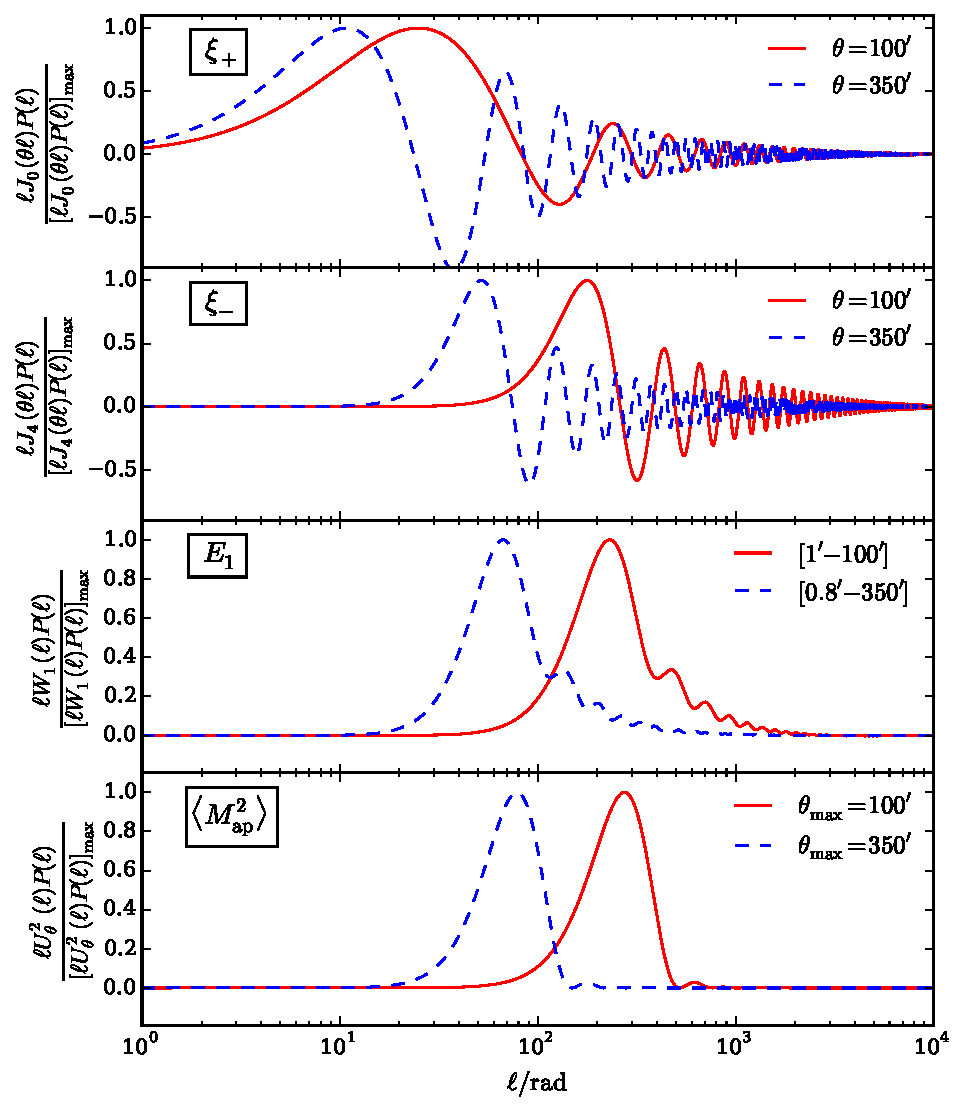
\includegraphics[width=0.60\textwidth]{figures/IntegAll.pdf} \\
\end{tabular}
\caption{\small{\label{fig:filters} 
Integrand of $\xi_+$ (upper), $\xi_-$
(upper middle), $E_1$ (lower middle, E-COSEBIs) and $\langle M_{\rm ap}
\rangle^2$ (lower panel). All integrands are of the form $\ell F(\ell)
P(\ell)$, where $F(\ell)$ is the corresponding weight-function for each
statistic and $P(\ell)$ is the E-mode convergence power spectrum, with the
exception of $\xi_\pm$, for which $P(\ell)$ is equal to the sum of the E and
B-mode power spectra. Two cases are shown for each statistic as listed in each
caption. For the aperture mass statistic $\theta_{\rm max}=2\theta$ is shown.
Note that higher order COSEBIs modes generally probe larger $\ell$-modes, hence
here we only show the lowest mode $E_1$. All values are normalized with respect
to their maximum value. This figure illustrates how different two-point cosmic shear
statistics have different dependences between the angular scales sampled and the $\ell$-range probed. }}
\end{center}
\end{figure}

